\chapter{Introduction}
\section*{Terminology}

\begin{wrapfigure}{r}{33 mm}
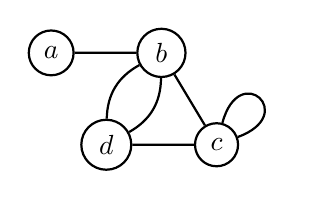
\begin{tikzpicture}[scale=1.4,
  thick,main node/.style={circle,draw,font=\sffamily\bfseries,minimum size=3mm}]

  \node[main node] (1) at (0,15/6) {$a$};
  \node[main node] (2) at (1,15/6){$b$};
  \node[main node] (11) at (1.5,10/6){$c$};
  \node[main node] (12) at (.5,10/6) {$d$};

  \path[every node/.style={font=\sffamily\small}]
   (11) edge [out=20,in=75,looseness=8] node[above] {} (11)
   (1) edge (2)
   (2) edge[bend left] (12)
   (2) edge[bend right] (12)
   (2) edge (11)
   (11) edge (12)
   (12) edge (12);
\end{tikzpicture}
\end{wrapfigure}

The diagram on the right may describe regular flights of an airline.
It has six flights which serve four airports labeled by $a$, $b$, $c$ and~$d$.

For this and similar type of data, mathematicians use the notion of \emph{pseudograph}.

Formally, a pseudograph is a finite nonempty set of \emph{vertexes}  (in our example a vertex is an airport) 
and finite collection of \emph{edges}, each edge connects two vertexes (in the example above, edge is a regular flight).
A pair of vertexes can be connected by few edges, such edges are called \emph{parallel} (in our example, it might mean that the airline makes few  flight a day between these airports). 
Also an edge can connect a vertex to itself, such edge is called a \emph{loop} (we might think of it as а sightseeing flight).

Thus, from mathematical point of view, the diagram above describes an example of pseudograph with vertexes $a$, $b$, $c$, $d$ and 
six edges; among them one loop at $c$ and a pair of parallel edges between $b$ and $d$.

\smallskip

The number of edges comming from one vertex is called its \emph{degree}, the loops are counted twice.
In the example above,
the degrees of $a,b,c$ and $d$ are $1,4,4$ и $3$ correspondingly.

A vertex with zero degree is called \emph{isolated} and a vertex of degree one is called \emph{end vertex}.

\smallskip

A pseudograph without loops is also called \emph{multigraph}.
A multigraph without parallel edges is also called \emph{graph}.
Most of the time we will work with graphs.

If $x$ and $y$ are vertexes of a pseudograph $G$, we say $x$ is \emph{adjacent} to $y$ if there is an edge between $x$ and $y$.
We say that a vertex $x$ is \emph{incident} with an edge $e$ if $x$ is an end vertex of $e$.

\section*{Wolf, goat and cabbage}

Usually we visualize the vertexes of a graph by points
and its edges are represented by a line connecting two vertexes.

However, the vertexes and edges of the graph might have a very different nature.
As an example, let us consider the following classical problem.

\begin{thm}{Problem}
A farmer purchased a wolf, a goat and a cabbage;
he needs to cross a river.
He has a boat, but he could carry only himself and a single one of his purchases: the wolf, the goat, or the cabbage.

If left unattended together, the wolf would eat the goat, or the goat would eat the cabbage.

The farmer has to carry himself and his purchases to the far bank of the river, leaving each purchase intact. How did he do it?
\end{thm}

\parit{Solution.}
Let us denote the farmer by $*$, the river by a vertical line $|$
the wolf by $w$, the goat by $g$ and the cabbage by $c$.
For example $wc|g{*}$ means that wolf and cabbage are on the left bank of the river and the goat with the farmer are on the right bank.

The starting position is $wgc{*}|$; that is, everyone is one the left bank.
The following graph describes all possible positions which can be achieved; each edge is labeled by the transported purchase.

\begin{center}
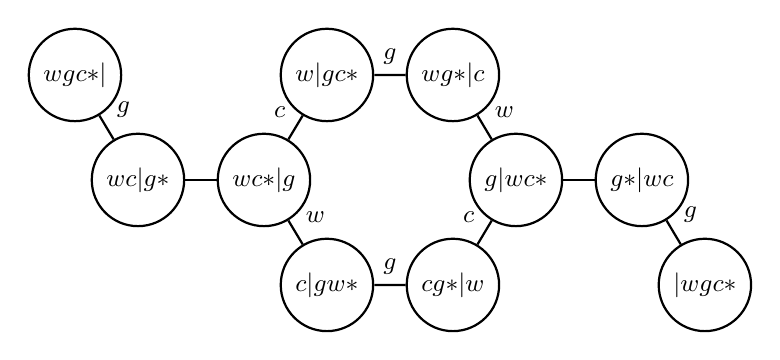
\begin{tikzpicture}[scale=1.6,
  thick,main node/.style={circle,draw,font=\sffamily\bfseries,minimum size=3mm}]

  \node[main node] (1) at (.5,5/6) {{\small${wgc{*}}|{}$}};
  \node[main node] (2) at (1,0){{\small${wc}|{g{*}}$}};
  \node[main node] (3) at (2,0){{\small${wc{*}}|{g}$}};
  \node[main node] (4) at (2.5,5/6){{\small${w}|{gc{*}}$}};
 \node[main node] (5) at (2.5,-5/6){{\small${c}|{gw{*}}$}};
  \node[main node] (6) at (3.5,-5/6){{\small${cg{*}}|{w}$}};
  \node[main node] (7) at (3.5,5/6){{\small${wg{*}}|{c}$}};
  \node[main node] (8) at (4,0){{\small${g}|{wc{*}}$}};
  \node[main node] (9) at (5,0){{\small${g{*}}|{wc}$}};
  \node[main node] (10) at (5.5,-5/6){{\small${}|{wgc{*}}$}};
  \path[every node/.style={font=\sffamily\small}]
   (1) edge node[auto]{$g$}(2)
   (2) edge node{}(3)
   (3) edge node[auto]{$c$}(4)
   (3) edge node[auto]{$w$}(5)
   (5) edge node[auto]{$g$}(6)
   (4) edge node[auto]{$g$}(7)
   (7) edge node[auto]{$w$}(8)
   (6) edge node[auto]{$c$}(8)
   (8) edge node[auto]{}(9)
   (9) edge node[auto]{$g$}(10);
\end{tikzpicture}
\end{center}

This graph shows that the farmer can achieve ${}|{wgc{*}}$ by legal moves.
It solves the problem, and also shows that there are exactly two different solutions;
assuming that the farmer does not want to repeat the same position twice. 
\qeds

Often graph comes with an extra structure, for example labeling of edges and/or vertexes as in the example above.

Here is a small variation of an other classical problem.

\begin{thm}{Problem} Missionaries and cannibals must cross a river using a boat which can carry at most two people, under the constraint that, for both banks, if there are missionaries present on the bank, they cannot be outnumbered by cannibals; the missionaries will be eaten otherwise.
The boat cannot cross the river by itself with no people on board.
\end{thm}

Let us introduce a notation to describe positions of missionaries, cannibals and the boat on the banks.
The river will be denoted by vertical line $|$;
let $*$ denotes the boat, we will write the number of cannibals on each side of $|$ and the number of missionaries by subscript. 
For example $4_2^*|0_2$ means that on the left bank we have four cannibals, two missionaries and the boat, and on the right bank there is no cannibals and two missionaries.

\begin{thm}{Exercise}
Assume four missionaries and four cannibals need to cross the river; in other words the beginning stage is $4_4^*|0_0$.
Draw a graph for all possible positions which can be achieved.

Conclude that all of them can not cross the river.
\end{thm}
